\documentclass[11pt,a4paper]{article}   

\usepackage{mathpazo}
\usepackage[T1]{fontenc}
\usepackage[utf8]{inputenc}

\usepackage{geometry}
\geometry{
	a4paper,
	left=25mm,
	top=20mm,
	bottom=20mm,
	right=25mm
}


\usepackage{float}
\usepackage{graphicx} 						
\usepackage{booktabs}
\usepackage{subcaption, multirow}

\usepackage{array}
\newcolumntype{x}[1]{>{\centering\arraybackslash}p{#1}}

\begin{document}

\title{Replication Exercise  \\ 
Cycles of Fire? Politics and Forest Burning in Indonesia}

\author{Sankalp Sharma}
\date{\today}

\maketitle

\section{Introduction}

The goal of this exercise is to replicate the figures and tables for the paper "Cycles of Fire? Politics and Forest Burning in Indonesia" by Clare Balboni, Robin Burgess, Anton Heil, Jonathan Old and Benjamin A. Olken. This paper exploits quasi-random variation in the timing of Indonesian district (kabupaten) elections to identify electoral cycles in forest fire activity. Following post-Soeharto decentralization reforms, substantial authority over land management devolved to district heads (bupati), whose elections were phased based on pre-1998 term expirations that create staggered, plausibly exogenous variation in electoral timing. 
\\
\\
Using satellite data on 107,000 fires from 2000–2016 and a Poisson event-study design, the authors show that both fire ignitions and burned area fall sharply in election years and spike immediately after. Specifically, ignitions rise by 56.8\% and burned area by 65.9\% in the year following elections, relative to the election year. These cycles are concentrated in “productive” forests (where land can be leased or converted for palm oil/logging), but absent in protected forests, consistent with political incentives to suppress illegal land clearing where regulatory discretion is highest and private rents largest. Fires following deforestation (“slash-and-burn”) shows similar dynamics, reinforcing that electoral suppression targets politically salient, human-driven activity. These findings contrast with standard political budget cycles where public spending rises pre-election and instead resemble cycles in enforcement of unpopular policies. 
\\
\\
The results imply that environmental degradation in decentralized regimes may be driven less by weak capacity and more by strategic leniency timed around electoral incentives. The paper contributes to a broader literature on the political economy of environmental enforcement, suggesting that institutional designs reducing local discretion may be important for mitigating externally costly but privately profitable ecological damage.
\\
\\
Overall, all the figures and tables replicated without any errors. 

\section{Main Figure}

\begin{figure}[H]
    \centering
    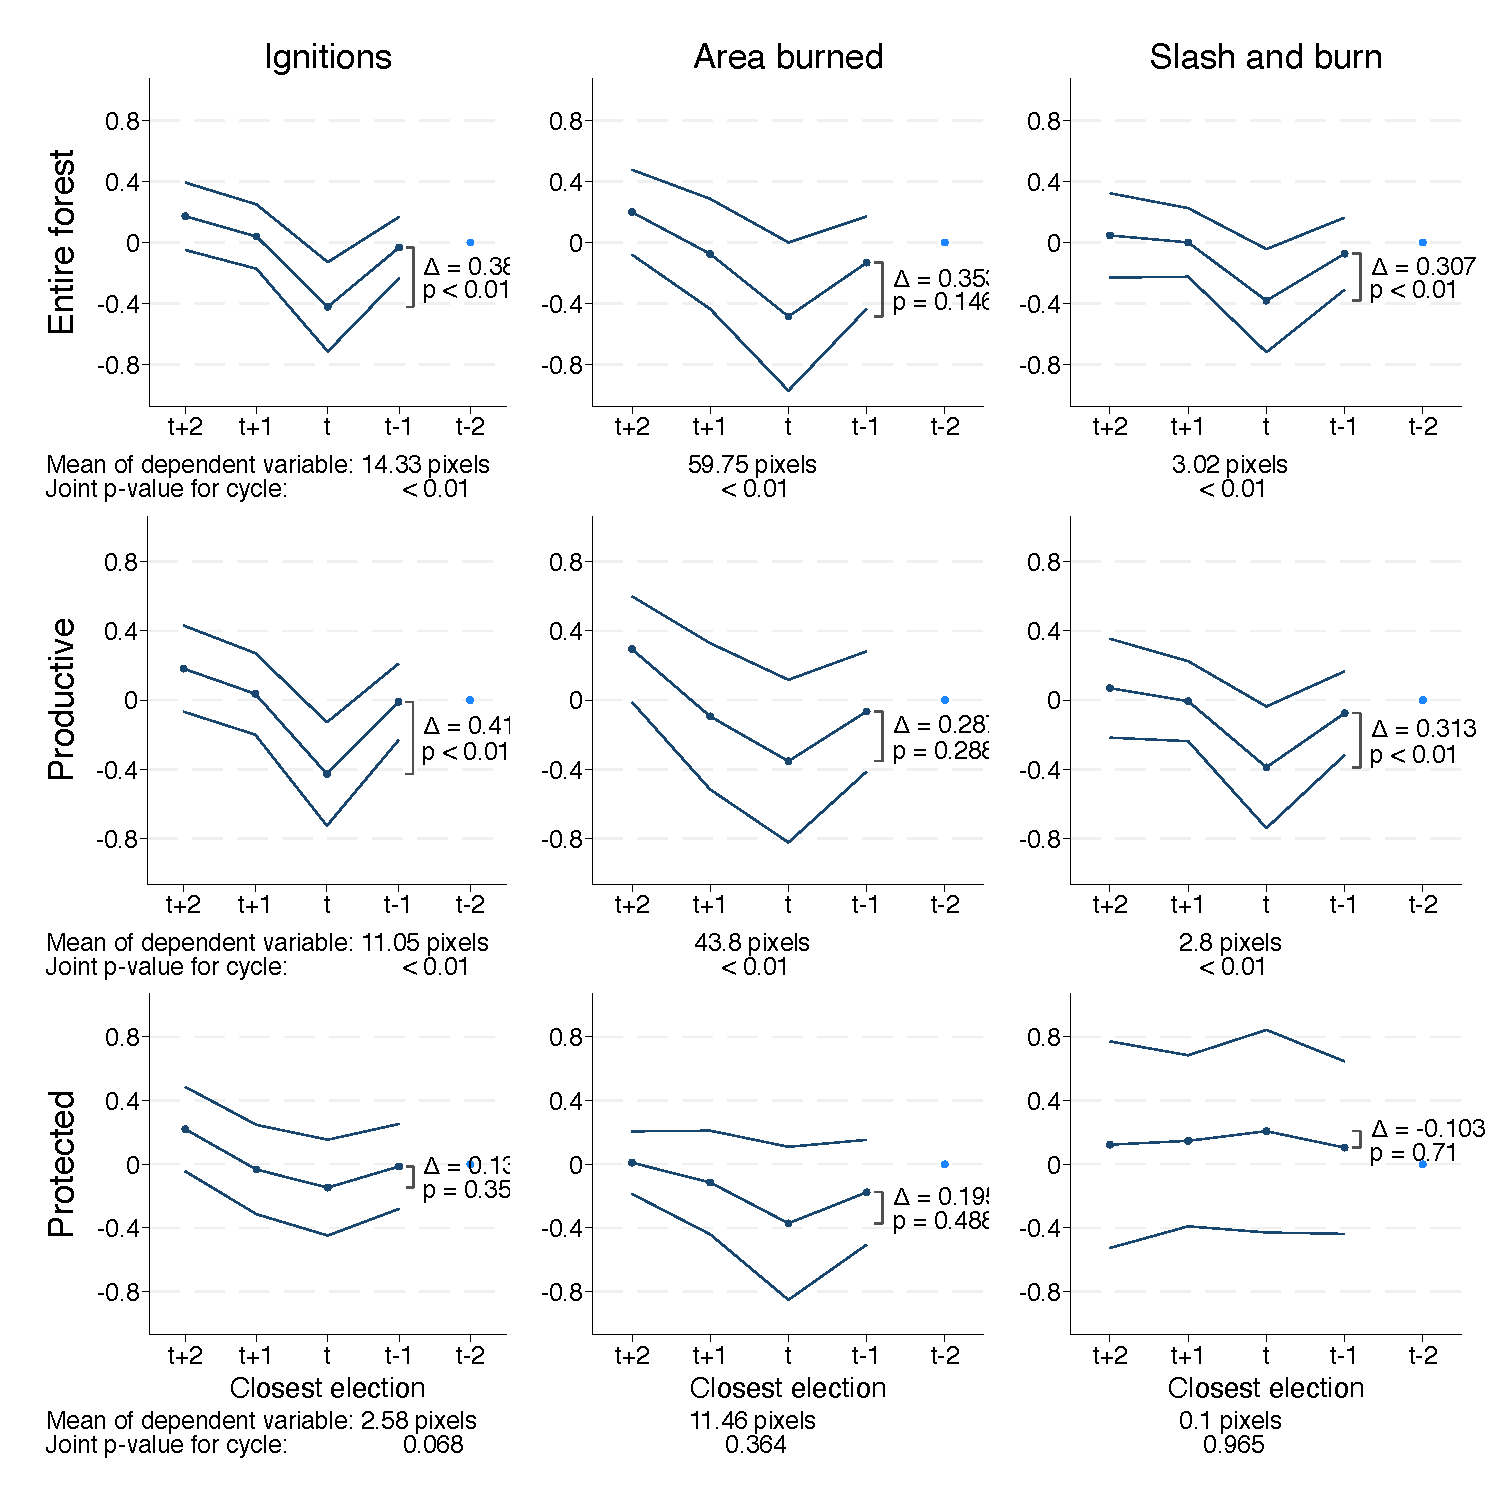
\includegraphics[width=1\linewidth]{../output/figures/figure_1.pdf}
\end{figure}

\appendix
\setcounter{section}{1}
\section{Full regression results by land types\label{sec:regtables}}
\setcounter{table}{0}
\renewcommand{\thetable}{B\arabic{table}}
\setcounter{figure}{0}
\renewcommand{\thefigure}{B\arabic{figure}}

\begin{table}[H]
	\centering
	\caption{Electoral cycle by land types -- Ignitions, District and Year FE}
	\scalebox{0.85}{%
	  \begin{tabular}{l *{7}{x{1.7cm}}}
		\toprule
		  & (1) & (2) & (3) & (4) & (5) & (6) & (7) \\
		  & All Forest & Concession & Oil Palm & Fibre & Logging & Unleased & Protected \\
		\midrule
		\textbf{Election date:}  \\
		\hspace{0.2cm} In 2 years&       0.104   &       0.092   &      -0.088   &       0.168   &       0.221   &       0.097   &       0.138   \\
                         &     (0.086)   &     (0.107)   &     (0.112)   &     (0.143)   &     (0.190)   &     (0.098)   &     (0.107)   \\
\hspace{0.2cm} Next year &       0.049   &       0.165   &       0.040   &       0.218   &       0.184   &      -0.049   &      -0.059   \\
                         &     (0.080)   &     (0.091)   &     (0.116)   &     (0.115)   &     (0.212)   &     (0.090)   &     (0.100)   \\
\hspace{0.2cm} This year &      -0.418   &      -0.378   &      -0.515   &      -0.328   &      -0.043   &      -0.441   &      -0.158   \\
                         &     (0.120)   &     (0.145)   &     (0.194)   &     (0.172)   &     (0.255)   &     (0.115)   &     (0.119)   \\
\hspace{0.2cm} Last year &       0.032   &       0.091   &       0.019   &       0.093   &       0.192   &      -0.049   &       0.078   \\
                         &     (0.083)   &     (0.107)   &     (0.152)   &     (0.110)   &     (0.163)   &     (0.076)   &     (0.115)   \\
\midrule \addlinespace Observations&        4218   &        4218   &        4218   &        4218   &        4218   &        4218   &        4218   \\
Mean of DV               &       17.63   &        9.04   &        4.00   &        4.13   &        0.90   &        6.92   &        3.37   \\
Spatial FE               &    District   &    District   &    District   &    District   &    District   &    District   &    District   \\
Temporal FE              &        Year   &        Year   &        Year   &        Year   &        Year   &        Year   &        Year   \\
Joint p-value            &\textless 0.01   &\textless 0.01   &\textless 0.01   &\textless 0.01   &       0.157   &\textless 0.01   &       0.149   \\
\textbf{This vs. last:} \\ \hspace{0.2cm} Difference&       0.450   &       0.469   &       0.534   &       0.420   &       0.235   &       0.392   &       0.236   \\
  \hspace{0.2cm} p-value &\textless 0.01   &\textless 0.01   &\textless 0.01   &\textless 0.01   &       0.138   &\textless 0.01   &       0.059   \\
\bottomrule
 \\ 
		\addlinespace
		\multicolumn{8}{l}{\footnotesize Note: Standard errors clustered at 2018 district level in parentheses.}
	  \end{tabular}%
	}
  \end{table}

\begin{table}[H]
	\centering
	\caption{Electoral cycle by land types -- Total area burned, District and Year FE}
	\scalebox{0.85}{%
\begin{tabular}{l x{1.7cm} x{1.7cm} x{1.7cm} x{1.7cm} x{1.7cm} x{1.7cm} x{1.7cm} }
\toprule
		& (1) & (2) & (3) & (4) & (5) & (6) & (7)  \\
	& All Forest & Concession & Oil Palm & Fibre & Logging & Unleased & Protected \\
 \midrule
 \textbf{Election date:}  \\
	\hspace{0.2cm} In 2 years&       0.163   &       0.160   &      -0.020   &       0.256   &       0.282   &       0.257   &      -0.173   \\
                         &     (0.152)   &     (0.209)   &     (0.148)   &     (0.300)   &     (0.240)   &     (0.147)   &     (0.151)   \\
\hspace{0.2cm} Next year &      -0.062   &       0.029   &      -0.116   &       0.037   &       0.180   &      -0.090   &      -0.226   \\
                         &     (0.143)   &     (0.199)   &     (0.212)   &     (0.237)   &     (0.245)   &     (0.143)   &     (0.144)   \\
\hspace{0.2cm} This year &      -0.541   &      -0.513   &      -0.370   &      -0.741   &      -0.055   &      -0.455   &      -0.420   \\
                         &     (0.201)   &     (0.251)   &     (0.237)   &     (0.313)   &     (0.328)   &     (0.182)   &     (0.226)   \\
\hspace{0.2cm} Last year &      -0.035   &       0.008   &      -0.014   &      -0.093   &       0.244   &      -0.075   &      -0.110   \\
                         &     (0.151)   &     (0.204)   &     (0.208)   &     (0.231)   &     (0.213)   &     (0.125)   &     (0.182)   \\
\midrule \addlinespace Observations&        4218   &        4218   &        4218   &        4218   &        4218   &        4218   &        4218   \\
Mean of DV               &       75.61   &       41.14   &       18.08   &       20.14   &        2.92   &       27.12   &       14.39   \\
Spatial FE               &    District   &    District   &    District   &    District   &    District   &    District   &    District   \\
Temporal FE              &        Year   &        Year   &        Year   &        Year   &        Year   &        Year   &        Year   \\
Joint p-value            &\textless 0.01   &       0.012   &       0.054   &\textless 0.01   &       0.063   &\textless 0.01   &       0.331   \\
\textbf{This vs. last:} \\ \hspace{0.2cm} Difference&       0.506   &       0.521   &       0.356   &       0.648   &       0.299   &       0.380   &       0.310   \\
  \hspace{0.2cm} p-value &\textless 0.01   &       0.021   &       0.114   &       0.031   &       0.098   &       0.042   &       0.213   \\
\bottomrule
 \\
\addlinespace
\multicolumn{8}{l}{Note: Standard errors clustered at 2018 district level in parentheses.}
 \end{tabular}%
	}
\end{table}


\begin{table}[H]
	\caption{Electoral cycle by land types -- Slash and burn, District and Year FE}
	\scalebox{0.85}{%
\begin{tabular}{l x{1.7cm} x{1.7cm} x{1.7cm} x{1.7cm} x{1.7cm} x{1.7cm} x{1.7cm} }
\toprule
		& (1) & (2) & (3) & (4) & (5) & (6) & (7)  \\
	& All Forest & Concession & Oil Palm & Fibre & Logging & Unleased & Protected \\
 \midrule
 \textbf{Election date:}  \\
	\hspace{0.2cm} In 2 years&       0.066   &       0.066   &      -0.179   &       0.121   &       0.364   &       0.088   &      -0.056   \\
                         &     (0.142)   &     (0.144)   &     (0.117)   &     (0.203)   &     (0.204)   &     (0.170)   &     (0.258)   \\
\hspace{0.2cm} Next year &       0.018   &       0.022   &      -0.131   &       0.092   &       0.083   &      -0.118   &       0.029   \\
                         &     (0.098)   &     (0.100)   &     (0.102)   &     (0.137)   &     (0.209)   &     (0.173)   &     (0.189)   \\
\hspace{0.2cm} This year &      -0.364   &      -0.353   &      -0.587   &      -0.241   &      -0.141   &      -0.620   &       0.045   \\
                         &     (0.143)   &     (0.145)   &     (0.170)   &     (0.182)   &     (0.281)   &     (0.197)   &     (0.268)   \\
\hspace{0.2cm} Last year &      -0.025   &      -0.014   &      -0.094   &      -0.048   &       0.131   &      -0.288   &       0.033   \\
                         &     (0.115)   &     (0.115)   &     (0.123)   &     (0.132)   &     (0.191)   &     (0.193)   &     (0.212)   \\
\midrule \addlinespace Observations&        4218   &        4218   &        4218   &        4218   &        4218   &        4218   &        4218   \\
Mean of DV               &        3.46   &        3.30   &        1.30   &        1.68   &        0.33   &        0.15   &        0.11   \\
Spatial FE               &    District   &    District   &    District   &    District   &    District   &    District   &    District   \\
Temporal FE              &        Year   &        Year   &        Year   &        Year   &        Year   &        Year   &        Year   \\
Joint p-value            &\textless 0.01   &\textless 0.01   &\textless 0.01   &       0.190   &       0.106   &\textless 0.01   &       0.973   \\
\textbf{This vs. last:} \\ \hspace{0.2cm} Difference&       0.338   &       0.339   &       0.494   &       0.192   &       0.272   &       0.332   &      -0.012   \\
  \hspace{0.2cm} p-value &\textless 0.01   &\textless 0.01   &\textless 0.01   &       0.119   &       0.196   &       0.020   &       0.956   \\
\bottomrule
 \\
\addlinespace
\multicolumn{8}{l}{Note: Standard errors clustered at 2018 district level in parentheses.}
 \end{tabular}%
 }
\end{table}

\begin{table}[H]
	\caption{Electoral cycle by land types -- Ignitions, District and Province $\times$ Year FE}
	\scalebox{0.85}{%
\begin{tabular}{l x{1.7cm} x{1.7cm} x{1.7cm} x{1.7cm} x{1.7cm} x{1.7cm} x{1.7cm} }
\toprule
		& (1) & (2) & (3) & (4) & (5) & (6) & (7)  \\
	& All Forest & Concession & Oil Palm & Fibre & Logging & Unleased & Protected \\
 \midrule
 \textbf{Election date:}  \\
	\hspace{0.2cm} In 2 years&       0.020   &       0.018   &      -0.123   &       0.226   &       0.030   &       0.022   &      -0.100   \\
                         &     (0.048)   &     (0.085)   &     (0.095)   &     (0.100)   &     (0.251)   &     (0.069)   &     (0.115)   \\
\hspace{0.2cm} Next year &      -0.033   &      -0.000   &       0.025   &       0.062   &      -0.332   &      -0.066   &      -0.063   \\
                         &     (0.056)   &     (0.058)   &     (0.076)   &     (0.087)   &     (0.233)   &     (0.078)   &     (0.113)   \\
\hspace{0.2cm} This year &      -0.014   &      -0.013   &      -0.133   &       0.181   &      -0.237   &      -0.083   &      -0.078   \\
                         &     (0.075)   &     (0.104)   &     (0.108)   &     (0.119)   &     (0.206)   &     (0.090)   &     (0.096)   \\
\hspace{0.2cm} Last year &       0.138   &       0.163   &       0.122   &       0.189   &       0.021   &       0.044   &       0.083   \\
                         &     (0.052)   &     (0.064)   &     (0.084)   &     (0.094)   &     (0.168)   &     (0.049)   &     (0.113)   \\
\midrule \addlinespace Observations&        4218   &        4218   &        4218   &        4218   &        4218   &        4218   &        4218   \\
Mean of DV               &       17.63   &        9.04   &        4.00   &        4.13   &        0.90   &        6.92   &        3.37   \\
Spatial FE               &    District   &    District   &    District   &    District   &    District   &    District   &    District   \\
Temporal FE              &   Prov-year   &   Prov-year   &   Prov-year   &   Prov-year   &   Prov-year   &   Prov-year   &   Prov-year   \\
Joint p-value            &\textless 0.01   &\textless 0.01   &       0.100   &       0.026   &       0.207   &       0.035   &       0.143   \\
\textbf{This vs. last:} \\ \hspace{0.2cm} Difference&       0.152   &       0.176   &       0.255   &       0.008   &       0.258   &       0.127   &       0.161   \\
  \hspace{0.2cm} p-value &       0.040   &       0.069   &       0.019   &       0.929   &       0.192   &       0.105   &       0.054   \\
\bottomrule
 \\
\addlinespace
\multicolumn{8}{l}{Note: Standard errors clustered at 2018 district level in parentheses.}
 \end{tabular}%
 }
\end{table}

\begin{table}[H]
	\caption{Electoral cycle by land types -- Total area burned, District and  Province $\times$ Year FE}
	\scalebox{0.85}{%
\begin{tabular}{l x{1.7cm} x{1.7cm} x{1.7cm} x{1.7cm} x{1.7cm} x{1.7cm} x{1.7cm} }
\toprule
		& (1) & (2) & (3) & (4) & (5) & (6) & (7)  \\
	& All Forest & Concession & Oil Palm & Fibre & Logging & Unleased & Protected \\
 \midrule
 \textbf{Election date:}  \\
	\hspace{0.2cm} In 2 years&       0.081   &       0.177   &      -0.078   &       0.614   &       0.034   &       0.140   &      -0.561   \\
                         &     (0.120)   &     (0.177)   &     (0.160)   &     (0.228)   &     (0.273)   &     (0.122)   &     (0.162)   \\
\hspace{0.2cm} Next year &      -0.118   &       0.012   &      -0.126   &       0.387   &      -0.542   &      -0.125   &      -0.278   \\
                         &     (0.110)   &     (0.121)   &     (0.164)   &     (0.174)   &     (0.294)   &     (0.128)   &     (0.169)   \\
\hspace{0.2cm} This year &       0.059   &       0.193   &       0.143   &       0.472   &      -0.327   &      -0.037   &      -0.378   \\
                         &     (0.144)   &     (0.206)   &     (0.216)   &     (0.283)   &     (0.232)   &     (0.153)   &     (0.163)   \\
\hspace{0.2cm} Last year &       0.190   &       0.279   &       0.134   &       0.465   &       0.048   &       0.059   &      -0.091   \\
                         &     (0.085)   &     (0.119)   &     (0.135)   &     (0.195)   &     (0.182)   &     (0.080)   &     (0.189)   \\
\midrule \addlinespace Observations&        4218   &        4218   &        4218   &        4218   &        4218   &        4218   &        4218   \\
Mean of DV               &       75.61   &       41.14   &       18.08   &       20.14   &        2.92   &       27.12   &       14.39   \\
Spatial FE               &    District   &    District   &    District   &    District   &    District   &    District   &    District   \\
Temporal FE              &   Prov-year   &   Prov-year   &   Prov-year   &   Prov-year   &   Prov-year   &   Prov-year   &   Prov-year   \\
Joint p-value            &       0.016   &       0.037   &       0.353   &       0.087   &       0.042   &       0.013   &\textless 0.01   \\
\textbf{This vs. last:} \\ \hspace{0.2cm} Difference&       0.130   &       0.087   &      -0.009   &      -0.007   &       0.374   &       0.096   &       0.287   \\
  \hspace{0.2cm} p-value &       0.374   &       0.652   &       0.969   &       0.970   &       0.082   &       0.450   &       0.044   \\
\bottomrule
 \\
\addlinespace
\multicolumn{8}{l}{Note: Standard errors clustered at 2018 district level in parentheses.}
 \end{tabular}%
 }
\end{table}

\begin{table}[H]
	\caption{Electoral cycle by land types -- Slash and burn, District and  Province $\times$ Year FE?}
	\scalebox{0.85}{%
\begin{tabular}{l x{1.7cm} x{1.7cm} x{1.7cm} x{1.7cm} x{1.7cm} x{1.7cm} x{1.7cm} }
\toprule
		& (1) & (2) & (3) & (4) & (5) & (6) & (7)  \\
	& All Forest & Concession & Oil Palm & Fibre & Logging & Unleased & Protected \\
 \midrule
 \textbf{Election date:}  \\
	\hspace{0.2cm} In 2 years&       0.078   &       0.076   &      -0.081   &       0.269   &      -0.021   &       0.045   &      -0.222   \\
                         &     (0.098)   &     (0.101)   &     (0.113)   &     (0.115)   &     (0.255)   &     (0.163)   &     (0.308)   \\
\hspace{0.2cm} Next year &      -0.013   &      -0.009   &      -0.090   &       0.167   &      -0.399   &      -0.314   &      -0.349   \\
                         &     (0.084)   &     (0.086)   &     (0.122)   &     (0.100)   &     (0.281)   &     (0.235)   &     (0.279)   \\
\hspace{0.2cm} This year &       0.001   &       0.013   &      -0.155   &       0.268   &      -0.509   &      -0.440   &       0.158   \\
                         &     (0.111)   &     (0.116)   &     (0.118)   &     (0.127)   &     (0.191)   &     (0.219)   &     (0.333)   \\
\hspace{0.2cm} Last year &       0.094   &       0.100   &       0.077   &       0.129   &      -0.163   &      -0.131   &      -0.518   \\
                         &     (0.066)   &     (0.067)   &     (0.107)   &     (0.090)   &     (0.192)   &     (0.195)   &     (0.204)   \\
\midrule \addlinespace Observations&        4218   &        4218   &        4218   &        4218   &        4218   &        4218   &        4218   \\
Mean of DV               &        3.46   &        3.30   &        1.30   &        1.68   &        0.33   &        0.15   &        0.11   \\
Spatial FE               &    District   &    District   &    District   &    District   &    District   &    District   &    District   \\
Temporal FE              &   Prov-year   &   Prov-year   &   Prov-year   &   Prov-year   &   Prov-year   &   Prov-year   &   Prov-year   \\
Joint p-value            &       0.083   &       0.124   &\textless 0.01   &       0.117   &       0.055   &\textless 0.01   &       0.022   \\
\textbf{This vs. last:} \\ \hspace{0.2cm} Difference&       0.094   &       0.086   &       0.232   &      -0.138   &       0.346   &       0.309   &      -0.676   \\
  \hspace{0.2cm} p-value &       0.389   &       0.448   &       0.091   &       0.109   &       0.175   &       0.019   &       0.025   \\
\bottomrule
 \\
\addlinespace
\multicolumn{8}{l}{Note: Standard errors clustered at 2018 district level in parentheses.}
 \end{tabular}%
 }
\end{table}

\begin{figure}[H]
	\caption{Electoral cycles in forest fires: No split children}
    \centering
    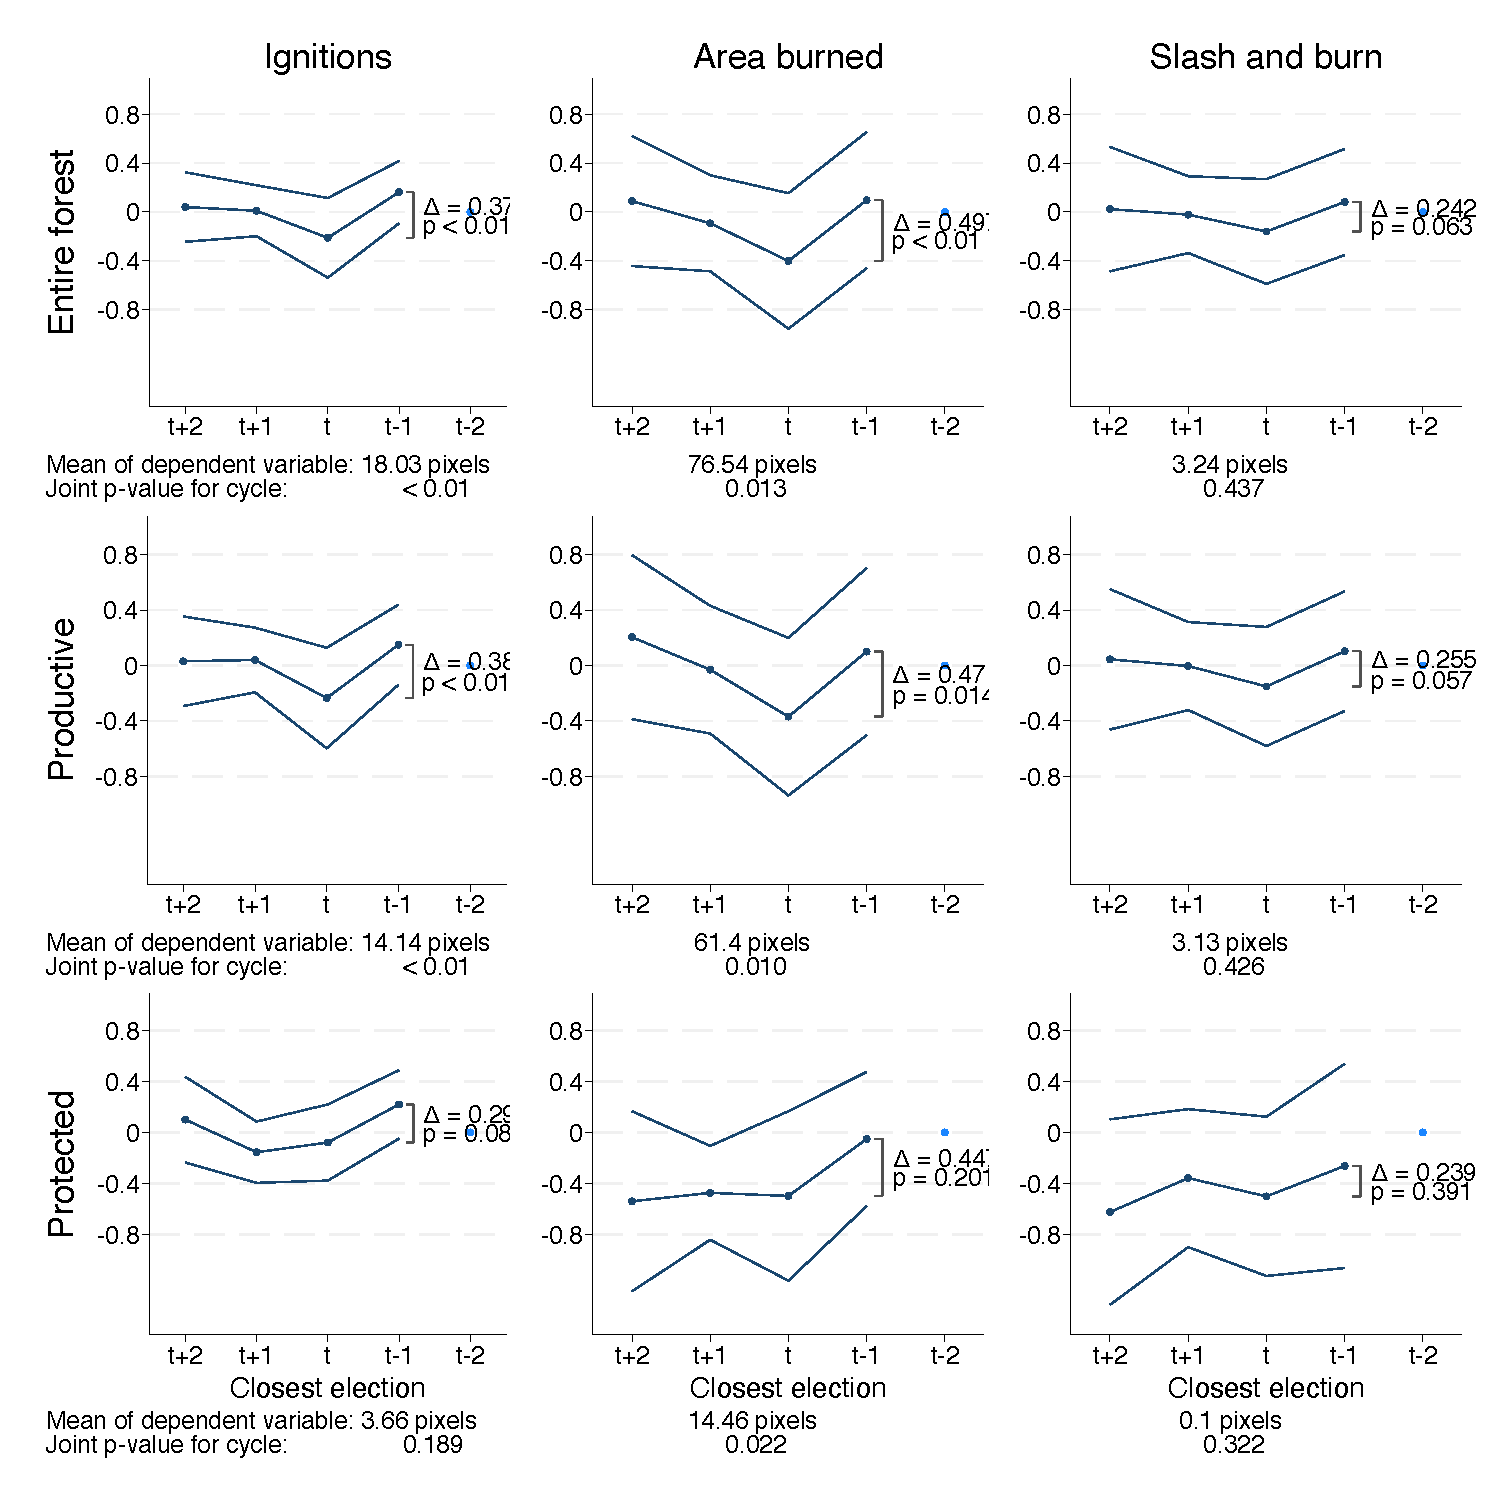
\includegraphics[width=1\linewidth]{../output/figures/figure_c1.pdf}
\end{figure}

\begin{figure}[H]
	\caption{Electoral cycles in forest fires: No parent districts}
    \centering
    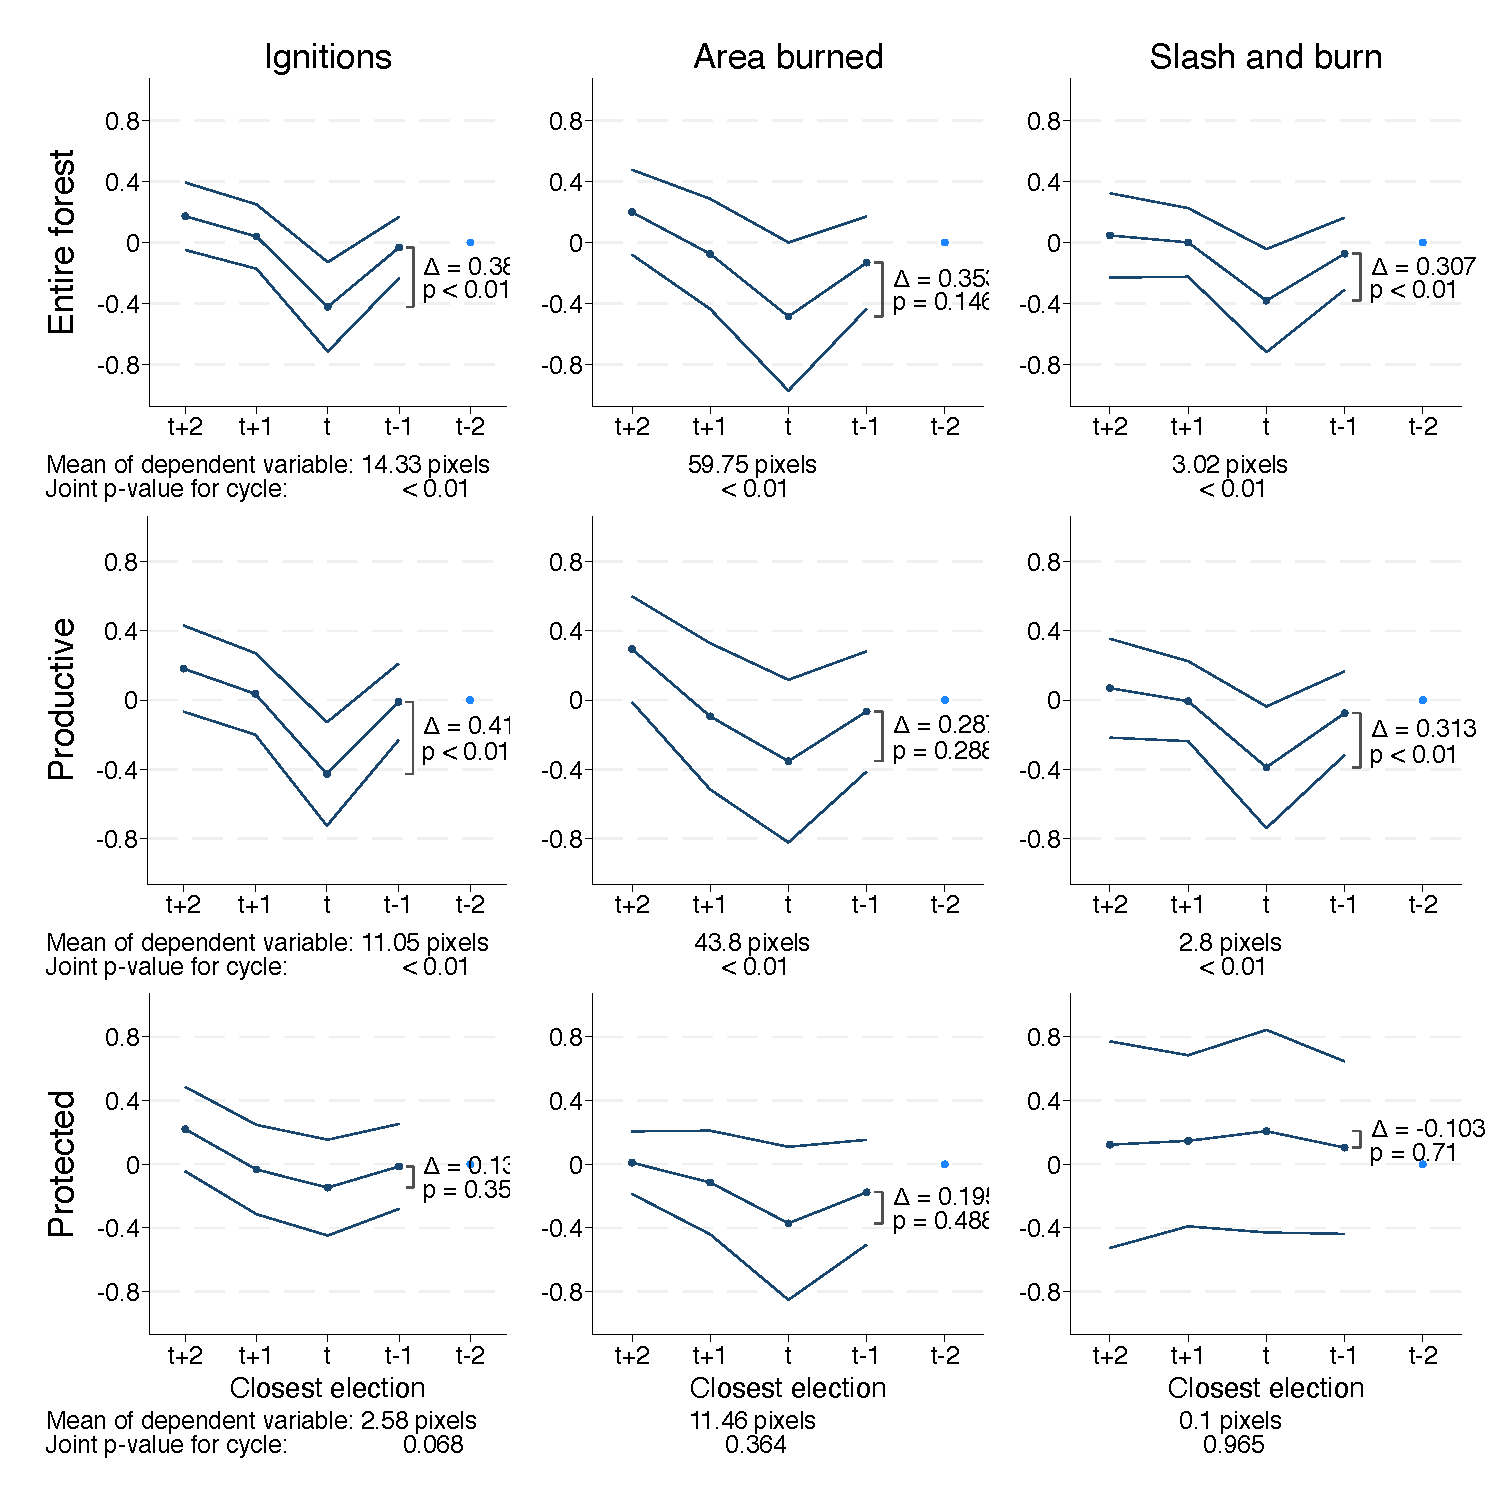
\includegraphics[width=1\linewidth]{../output/figures/figure_c2.pdf}
\end{figure}

\end{document}